\begin{figure*}[htbp]
    \centering%
    \setlength{\tabcolsep}{0.002\textwidth}%
    \renewcommand{\arraystretch}{1}%
    \footnotesize%
    \begin{tabular}{cccccccc}
        &Initial asset& \multicolumn{6}{c}{
            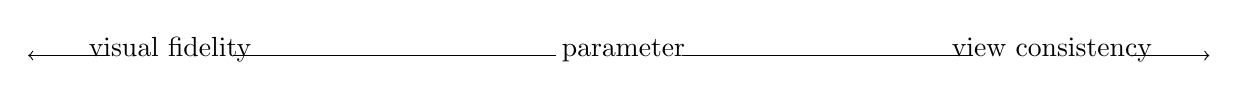
\begin{tikzpicture}
                \draw[<-] (0,0) -- (1,0);
                \draw[-] (2.6,0) -- (6.7,0);
                \draw[-] (8.3,0) -- (12,0);
                \draw[->] (14,0) -- (15,0);
                \node[above] at (1.8,-0.2) {visual fidelity};
                \node[above] at (7.5,-0.2) {$\bias$ parameter};
                \node[above] at (13,-0.2) {view consistency};
            \end{tikzpicture}
        }\\[-4pt]%
        && 0.0 & 0.6 & \textbf{1.2} & \textbf{1.8} & 2.4 & 3.0\\%
        \rotatebox{90}{\hspace*{4em}View 1}&%
        \includegraphics[height=0.14\linewidth, trim=150 0 100 0, clip]{figures/hparams_adjusting/initial_2_overlay.jpg}&%
        \includegraphics[height=0.14\linewidth, trim=200 40 300 460, clip]{figures/hparams_adjusting/0.0_2_overlay.jpg}&%
        \includegraphics[height=0.14\linewidth, trim=200 40 300 460, clip]{figures/hparams_adjusting/0.6_2_overlay.jpg}&%
        \includegraphics[height=0.14\linewidth, trim=200 40 300 460, clip]{figures/hparams_adjusting/1.2_2_overlay.jpg}&%
        \includegraphics[height=0.14\linewidth, trim=200 40 300 460, clip]{figures/hparams_adjusting/1.8_2_overlay.jpg}&%
        \includegraphics[height=0.14\linewidth, trim=200 40 300 460, clip]{figures/hparams_adjusting/2.4_2_overlay.jpg}&%
        \includegraphics[height=0.14\linewidth, trim=200 40 300 460, clip]{figures/hparams_adjusting/3.0_2_overlay.jpg}\\%
        \rotatebox{90}{\hspace*{2em}View 2, $+ 40^\circ$}&
        \includegraphics[height=0.14\linewidth, trim=150 0 100 0, clip]{figures/hparams_adjusting/initial_3_overlay.jpg}&%
        \includegraphics[height=0.14\linewidth, trim=200 40 300 460, clip]{figures/hparams_adjusting/0.0_3_overlay.jpg}&%
        \includegraphics[height=0.14\linewidth, trim=200 40 300 460, clip]{figures/hparams_adjusting/0.6_3_overlay.jpg}&%
        \includegraphics[height=0.14\linewidth, trim=200 40 300 460, clip]{figures/hparams_adjusting/1.2_3_overlay.jpg}&%
        \includegraphics[height=0.14\linewidth, trim=200 40 300 460, clip]{figures/hparams_adjusting/1.8_3_overlay.jpg}&%
        \includegraphics[height=0.14\linewidth, trim=200 40 300 460, clip]{figures/hparams_adjusting/2.4_3_overlay.jpg}&%
        \includegraphics[height=0.14\linewidth, trim=200 40 300 460, clip]{figures/hparams_adjusting/3.0_3_overlay.jpg}\\%
    \end{tabular}%
    \caption{The bias parameter $\bias$ trades between visual fidelity (left insets) and multi-view consistency (right insets). The first column shows the initial asset in two views that condition the diffusion model. The white shapes outline a UV region, which we analyze in the insets to illustrate the impact of the $\bias$ parameter on generated visuals.
    Values between 1.2 and 1.8 strike a good balance in this particular scene.}
    \label{fig:hparams}
\end{figure*}









